\chapter{Introduction to Mobile Computing} 

\section{Aims}
\paragraph{} At the end of this topic you will be able to:

\begin{itemize}
\item Explain where ‘mobile app’ development fits into the recent history of computing \& mobile computing. 
%\item Develop an Android app % In 2016 will include Hello Android but not in 2015
\end{itemize}


\section{The Rise of Mobile Computing}
\paragraph{} Today's mobile phone owes its origins to radio phones which were introduced on first class passenger trains in Germany in 1926. Mobile technology was enhanced during WW2 when Motorola created a walkie-talkie for the US Army – which was carried in a backpack to house the huge batteries.

\paragraph{} Following the development of cell-based transmitters and receivers in the late 1940s, the 1950s saw car phones making use of this cell technology although calls were not continuous as the car travelled from one cell to the next.

\paragraph{} In 1956 Ericsson created the first system that did not require manual control in the base stations in Sweden. Unfortunately the phone weighed 40 kilograms so not mobile in the sense we understand today.

\paragraph{} Until 1970 mobile technologies continued to be developed mainly in US and USSR. In 1971 an engineer from Bell Labs found a solution for transferring the call from a network to another without loss of communication. In 1973 Motorola made its first call on a truly mobile phone, illustrated in Figure \ref{fig:brick-phone}, – which is now referred to as the first generation. After specialising in military communications, Vodaphone launched the UKs mobile network in 1985. By the mid to late 1980s the mobile phone was the must have status symbol of business wheelers and dealers in Thatcherite Britain.

\begin{figure}[htb]
\centering
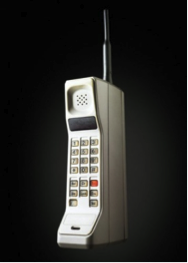
\includegraphics[width=0.5\textwidth]{images/brick-phone}
\caption{Motorola's mass marketed phone from 1973}
\label{fig:brick-phone}
\end{figure}

\paragraph{} In the 1990s the second generation of phones appeared – introducing digital technology in the form of GSM (Global System for Mobile communications) into the networks. In Europe Nokia was a key developer of GSM and the first GSM network was opened in Finland. This second generation of mobile phones introduced the SMS service – arguably the start of social networking. Customisation started here – with downloadable, if expensive, ring tones – and business users were overtaken by the general population driven by a huge interest from younger users.

\paragraph{} Third generation networks \& devices appeared in Japan in 2001. The main aim was to satisfy the demand for data services  i.e. move to packet switching to speed things up so we could get internet-on-the-go, swap photos and video. The i) mobile phone and ii)PDAs/ netbooks with dongles started to converge with the smartphone emerging as the product of their convergence. 

\paragraph{} The fourth generation is fast approaching – VoIP will replace traditional circuit switched calls in a network optimised for data services. At the moment it’s just a marketing term.

\section{Recent History of Mobile Computing}

\begin{itemize}

\item The first commercial laptop illustrated in Figure \ref{fig:grid-compass}, the GRiD Compass\footnote{\url{http://en.wikipedia.org/wiki/Grid_Compass}} started selling in 1982 at a price tag of \$8000 the main customer was the US Department of Defence and NASA.

\item Personal Digital Assistant was a term used to describe the Apple Newton  illustrated in Figure \ref{fig:apple-newton}, first sold in 1992. PDAs could keep calendars, play games, synch with your desktop. Although there was a proliferation of manufacturers' operating systems, the Symbian OS came to dominate, with MS following with their Microsoft CE OS.

\item The Nokia 9000  illustrated in Figure \ref{fig:nokia-9000}, was released 1996. A phone which could send/receive emails and type up Word docs. Arguably the world's first smartphone.

\item In 2002, Blackberry manufacturers Re-search in Motion (RIM) released their first smartphone,  illustrated in Figure \ref{fig:rim-blackberry}, following their successful push email technology. Popular amongst business users originally, the Blackberry found a new market amongst teenage girls thanks to the BlackBerry Messenger app, before declining in popularity.

\item The first Apple iPhone, illustrated in Figure \ref{fig:apple-iPhone}, was released in June 2007. The latest version, 4, was released in July 2010 (following the iPad release in April 2010). The iPhone was the first smartphone with mass market appeal.

\item In October 2008, the first Android phone – the HTC Dream (aka T-Mobile G1), illustrated in Figure \ref{fig:android-phone}, – was released. This was followed by the HTC Hero and now HTC Desire \& Samsung Galaxy, among others. Encouraged by the open nature of the development kit, this is creating a garage app developer culture.

\end{itemize}

\begin{figure}[htb]
        \centering
        \begin{subfigure}[b]{0.3\textwidth}
                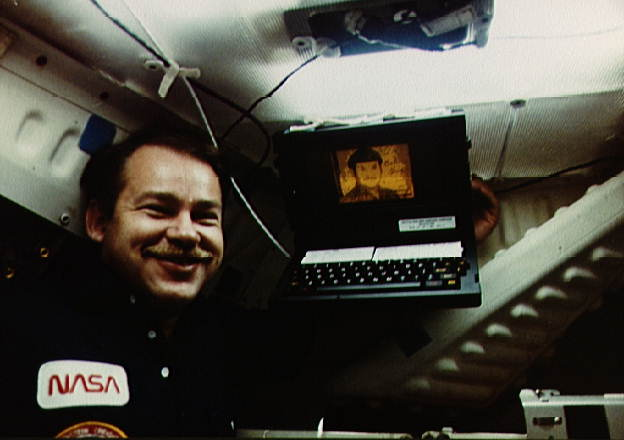
\includegraphics[width=\textwidth]{images/grid-compass}
                \caption{GRiD Compass}
                \label{fig:grid-compass}
        \end{subfigure}%
        ~ %add desired spacing between images, e. g. ~, \quad, \qquad, \hfill etc.
          %(or a blank line to force the subfigure onto a new line)
        \begin{subfigure}[b]{0.3\textwidth}
                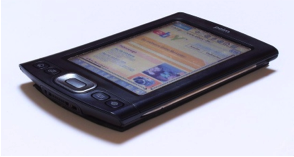
\includegraphics[width=\textwidth]{images/apple-newton}
                \caption{Apple Newton}
                \label{fig:apple-newton}
        \end{subfigure}
        ~ %add desired spacing between images, e. g. ~, \quad, \qquad, \hfill etc.
          %(or a blank line to force the subfigure onto a new line)
        \begin{subfigure}[b]{0.3\textwidth}
                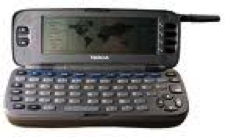
\includegraphics[width=\textwidth]{images/nokia-9000}
                \caption{Nokia 9000}
                \label{fig:nokia-9000}
        \end{subfigure}
        \caption{The GRiD Compass, Apple Newton, \& Nokia 9000}\label{fig:early-mobile-platforms-1}
\end{figure}

\begin{figure}[htb]
        \centering
        \begin{subfigure}[b]{0.3\textwidth}
                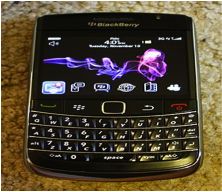
\includegraphics[width=\textwidth]{images/rim-blackberry}
                \caption{RIM Blackberry}
                \label{fig:rim-blackberry}
        \end{subfigure}%
        ~ %add desired spacing between images, e. g. ~, \quad, \qquad, \hfill etc.
          %(or a blank line to force the subfigure onto a new line)
        \begin{subfigure}[b]{0.3\textwidth}
                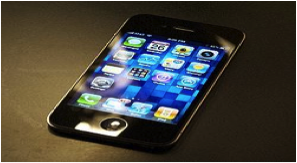
\includegraphics[width=\textwidth]{images/apple-iphone}
                \caption{Apple iPhone}
                \label{fig:apple-iPhone}
        \end{subfigure}
        ~ %add desired spacing between images, e. g. ~, \quad, \qquad, \hfill etc.
          %(or a blank line to force the subfigure onto a new line)
        \begin{subfigure}[b]{0.3\textwidth}
                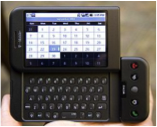
\includegraphics[width=\textwidth]{images/android-phone}
                \caption{Android Phone}
                \label{fig:android-phone}
        \end{subfigure}
        \caption{The Blackberry, iPhone, \& Android}\label{fig:early-mobile-platforms-1}
\end{figure}



\paragraph{} \emph{Where are we now?} The line between communication and computation has become increasingly blurred. A smartphone is now a handheld computer with integrated mobile phone (and pager, compass, camera, GPS, torch, ...)

\begin{quote}
"I have always wished for my computer to be as easy to use as my telephone; my wish has come true because I can no longer figure out how to use my telephone." 
— Bjarne Stroustrup  (Danish inventor of C++)
\end{quote}

\paragraph{} What do we expect of our mobile computing devices?
\begin{itemize}
\item phone
\item touchscreen or at least easy character entry
\item email
\item camera \& memory to save photos
\item audio \& video recorder \& player
\item web browsing
\item app platform eg games
\item reasonable battery life
\item small?
\end{itemize}

\paragraph{} Less discerning about:
\begin{itemize}
\item price - not necessarily cost conscious, at the moment
\item shelf life
\end{itemize}

\paragraph{} So what's the current state of play? Check with Gartner, market analysts. Android phones and iPhones continue to increase their market share.  New markets include the developing world – Huawei Telecom in China are manufacturing cheap Androids for India and Africa. There is also growth in iPad/ Android tablets.
 

 %%
 %%
 %% INSERT SECTION ON GARTNER SALES FIGURES
 %%
 %%
 %%


 \paragraph{} To a large extent the availability of apps is driving these increases for the iPhone and Android. Blackberry launched their own apps market and saw some growth in their handset sales. Meanwhile Symbian have opened up their OS. Huawai Telecom have launched a cheap Android phone in India – the Ideo. It’s hard to see a way for the iPhone to reach the developing world.


\section{Summary}
\paragraph{} In this topic we have attempted to understand why mobile computing and communication have become popular now by studying longer term trends in the wider fields of computing and communication.

\section{Directed Study}
\paragraph{} 

\begin{itemize}
\item Read Chapters 1 to 3 of Android Wireless Application Development \cite{conder_2010_android_ebook}.
\item Read more about the history of mobile computing, for example the Wikipedia page on the history of mobile phones is a good place to start\footnote{\url{http://en.wikipedia.org/wiki/History_of_mobile_phones}}.
\item Visit the developers website http://developer.android.com
\item Check your understanding of the topic by answering the following:
\begin{enumerate}
\item Name three apps you have used/ heard about and identify the platform they run on?
\item What makes a good app?
\item In Android-speak, what is an activity?
\item How do Intents work?
\end{enumerate}
\item If you have access to a computer at home, download and install the Oracle Java JDK\footnote{\url{http://www.oracle.com/technetwork/java/javase/downloads/index.html}} then install the Android development tools\footnote{\url{http://developer.android.com/sdk/index.html}}.
\item Have a look at the App Inventor\footnote{\url{http://appinventor.mit.edu/}}  – what do you think – can this revolutionise app development? It was initially developed by Google then, when abandoned, MIT stepped in.
\end{itemize}


%\section{Resources}

